\documentclass[10pt,a4paper]{article}
\usepackage[margin=1.8cm]{geometry}
\usepackage[LGR,T1]{fontenc}
\usepackage[utf8]{inputenc}
\usepackage{lmodern}
\usepackage[english,greek]{babel}
\usepackage{microtype}
\usepackage{graphicx}
\usepackage{booktabs}
\usepackage{amsmath}
\usepackage{caption}
\usepackage{enumitem}
\usepackage[hidelinks,bookmarks=false]{hyperref}
\captionsetup{font=small,labelfont=bf,skip=3pt}
\setlist{nosep,leftmargin=1.2em}
\setlength{\parskip}{2pt}
\setlength{\textfloatsep}{8pt}
\setlength{\floatsep}{6pt}

% Latin text inside Greek: \en{...} for words, \texttt is always Latin
\newcommand{\en}[1]{\textlatin{#1}}
\let\origtexttt\texttt
\renewcommand{\texttt}[1]{\textlatin{\origtexttt{#1}}}

\title{\vspace{-1.2cm}\Large\textbf{Εργασία 1: Κλίση του \en{t-SNE} σε γράφους με \en{Barnes--Hut}}\\[2pt]
\large Παράλληλα και Διανεμημένα Συστήματα Υπολογιστών, ΑΠΘ, 2026}
\author{Αθανάσιος Καρατζάς (ΑΕΜ 10514)\\
\small Κώδικας και δεδομένα: \en{\url{https://github.com/thkaratzas/graph-t-sne-Karatzas}}}
\date{\vspace{-0.6cm}}

\begin{document}
\maketitle

\section{Τι υπολογίζεται}

Για έναν γράφο με βάρη $W$ υπολογίζω μία κλίση του \en{t-SNE},
$\partial C/\partial y_i = 4(F^{\mathrm{attr}}_i - F^{\mathrm{rep}}_i)$, στο δοσμένο $Y_0$,
σε τέσσερα βήματα: (1) τις πιθανότητες $P$, (2) την έλξη κατά μήκος των ακμών,
(3) την άπωση και το $Z$ με \en{quadtree} και \en{Barnes--Hut} ($\theta=0.5$),
(4) την κλίση. Κάθε βήμα υπάρχει σε τέσσερις εκδόσεις: σειριακή, \en{OpenMP}, \en{OpenCilk} και
\en{Pthreads}. Όλα τα αρχεία μοιράζονται ένα \en{header} (\texttt{tsne.h}) και μερικά κοινά κομμάτια
(\texttt{p\_common.c}, \texttt{quadtree.c}, \texttt{bh\_common.c}), και κάθε έκδοση προσθέτει μόνο
τους δικούς της παράλληλους βρόχους.

\section{Δομές δεδομένων και αλγόριθμοι}

\textbf{Αραιός πίνακας.} Ο $W$ διαβάζεται με τον \en{reader} του \en{starter} σε μορφή \en{CSC} με
δείκτες από το 0. Επειδή ο $W$ είναι συμμετρικός, η στήλη $i$ είναι και γραμμή $i$, οπότε τον
χρησιμοποιώ ως \en{CSR}: οι γείτονες του $i$ είναι τα \texttt{row[k]} για
$k\in[\texttt{colptr}[i],\texttt{colptr}[i+1])$. Ο $P$ έχει την ίδια δομή, οπότε είναι ένας πίνακας
\texttt{P[nnz]} στοιχισμένος με το \texttt{W.val}, χωρίς νέους πίνακες δεικτών. Στην αρχή το πρόγραμμα
ελέγχει ότι οι γραμμές είναι ταξινομημένες, ότι τα βάρη είναι θετικά και ότι η δομή είναι
συμμετρική, γιατί ο υπόλοιπος κώδικας στηρίζεται σε αυτά τα τρία.

\textbf{Βήμα 1, $P$.} Για τη γραμμή $i$ αποθηκεύω $\ell_k=\log(w_k/w_{\max})\le 0$, ώστε το
$p_k\propto e^{\beta\ell_k}\le 1$ να μην υπερχειλίζει ποτέ, και η εντροπία είναι
$H(\beta)=\log S-\beta\sum_k e^{\beta\ell_k}\ell_k/S$ με $S=\sum_k e^{\beta\ell_k}$.
Η $H$ φθίνει ως προς $\beta$, οπότε κάνω διχοτόμηση: ξεκινώ από $\beta=1$, διπλασιάζω μέχρι η $H$
να πέσει κάτω από $\log\min(u,d_i)$ και μετά υποδιπλασιάζω το διάστημα, μέχρι
$|H-\log\min(u,d_i)|<10^{-5}$ ή 200 βήματα. Γραμμές με ίσα βάρη ή με $u\ge d_i$ μένουν ομοιόμορφες
($\beta=0$). Για τη συμμετρικοποίηση $p_{ij}=(p_{j|i}+p_{i|j})/2n$ το στοιχείο $(j,i)$ βρίσκεται με
δυαδική αναζήτηση στη γραμμή $j$.

\textbf{Βήμα 2, έλξη.} Ένα πέρασμα ανά γραμμή:
$F^{\mathrm{attr}}_i=\sum_{j}p_{ij}(1+d_{ij}^2)^{-1}(y_i-y_j)$, δηλαδή το γινόμενο $Y(D-A)$ χωρίς
να σχηματιστούν οι $A$ και $D$. Κάθε γραμμή γράφει μόνο το $F_i$, άρα οι γραμμές είναι ανεξάρτητες.

\textbf{Βήμα 3, \en{quadtree}.} Προσαρμοστικό δέντρο με χωρητικότητα φύλλου $m$. Οι δείκτες των
σημείων βρίσκονται σε έναν πίνακα \texttt{perm}, και κάθε κελί κατέχει ένα συνεχές κομμάτι του.
Ο χωρισμός ενός κελιού είναι ένα \en{counting sort} σε τέσσερα τεταρτημόρια (μέτρηση,
\en{prefix sum}, μεταφορά σε \en{buffer}, αντιγραφή πίσω). Τα κελιά είναι ξεχωριστοί κόμβοι με
\texttt{malloc} και τέσσερις δείκτες σε παιδιά, ώστε τα τέσσερα υποδέντρα να χτίζονται ταυτόχρονα
χωρίς να μοιράζονται τίποτα. Τα κέντρα μάζας υπολογίζονται σε ξεχωριστό πέρασμα, από κάτω προς τα
πάνω. Το \en{walk} για το σημείο $i$ αντιμετωπίζει ένα κελί ως ένα σημείο με μάζα $N_{\mathrm{cell}}$
όταν $r_{\mathrm{cell}}<\theta\,|y_i-y_{\mathrm{cell}}|$, όπου $r_{\mathrm{cell}}$ είναι η
\emph{διαγώνιος} $2h\sqrt2$. Αλλιώς ανοίγει το κελί, και σε φύλλο προσθέτει τα σημεία ένα-ένα,
παραλείποντας το $i$. Η μη κανονικοποιημένη άπωση και το $Z$ αθροίζονται στο ίδιο \en{walk}, και στο
τέλος το $F$ διαιρείται με το $Z$. Ένα κελί που περιέχει το $y_i$ έχει πάντα
$|y_i-y_{\mathrm{cell}}|\le r_{\mathrm{cell}}$, άρα για $\theta<1$ ανοίγει πάντα, και το $i$ μπορεί
να συναντήσει τον εαυτό του μόνο μέσα σε φύλλο.

\textbf{Ταυτισμένα σημεία.} Στα \texttt{com-Amazon} και \texttt{coPapersDBLP} το δέντρο έφτασε σε
βάθος 50 για κάθε $m$ έως 32. Ένας διαγνωστικός έλεγχος που μετρά τα φύλλα στο όριο βάθους έδειξε
1583 τέτοια φύλλα με 38\,605 σημεία (7.1\%) στο \en{DBLP}, με έως 114 σημεία σε ένα φύλλο, και 276
σημεία στο \en{Amazon}. Είναι σημεία με την ίδια θέση στο $Y_0$. Η εκτίμησή μου είναι ότι κόμβοι με
ίδιες γειτονιές (κλίκες από \en{papers} με τους ίδιους συγγραφείς) κατέρρευσαν στο ίδιο σημείο στις
300 επαναλήψεις. Τέτοια σημεία δεν χωρίζονται, οπότε χωρίς όριο βάθους η αναδρομή της κατασκευής δεν
τελειώνει ποτέ. Κρατώ \texttt{MAX\_DEPTH = 50}. Μέσα σε ένα τέτοιο φύλλο τα ζεύγη δίνουν $q=1$ και
μηδενική δύναμη, δηλαδή ακριβώς τον τύπο για $j\ne i$, άρα το αποτέλεσμα μένει σωστό.

\textbf{Επιλογή του $m$.} Δοκίμασα $m\in\{1,2,4,8,16,32\}$ (3 εκτελέσεις για το καθένα,
\texttt{results/sweep\_m.csv}). Μικρό $m$ σημαίνει πολλά κελιά και πολλά άλματα σε δείκτες, ενώ μεγάλο
$m$ σημαίνει περισσότερα ακριβή ζεύγη ανά φύλλο. Το σφάλμα δεν άλλαξε με το $m$ (το καθορίζει το
$\theta$), μόνο ο χρόνος. Το $m=16$ ήταν το ταχύτερο στους δύο μεγάλους γράφους (\en{build+com+walk}
2.79\,\en{s} και 3.61\,\en{s} στο μηχάνημα ανάπτυξης, έναντι 3.03\,\en{s} και 3.73\,\en{s} για $m=8$).
Στο \texttt{k49} οι διαφορές ανάμεσα στα 8, 16 και 32 ήταν μέσα στον θόρυβο. Χρησιμοποιώ $m=16$.

\section{Παραλληλοποίηση}

\begin{table}[h]
\centering\small
\begin{tabular}{@{}p{2.2cm}p{4.3cm}p{4.3cm}p{5.0cm}@{}}
\toprule
 & \en{OpenMP} & \en{OpenCilk} & \en{Pthreads} \\
\midrule
$P$, έλξη, κλίση & \texttt{parallel for schedule(runtime)} & \texttt{cilk\_for}, \en{grainsize} 256 & δική μου \texttt{pt\_for}: στατικά \en{blocks} ή δυναμικά κομμάτια από έναν \en{atomic} μετρητή \\
\en{buffer} για τον $P$ & ένα ανά \en{thread} μέσα στο \texttt{parallel} & το κομμάτι της ίδιας της γραμμής στο $p_{j|i}$ & το κομμάτι της ίδιας της γραμμής στο $p_{j|i}$ \\
κατασκευή δέντρου, κέντρα μάζας & \en{tasks} για παιδιά με $>10^4$ σημεία, \texttt{taskwait} & \texttt{cilk\_spawn} με το ίδιο όριο, \texttt{cilk\_sync} & νέο \en{thread} ανά παιδί έως βάθος $\lceil\log_4 p\rceil$, μετά αναδρομή \\
\en{walk}, άμεσος υπολογισμός & \texttt{reduction(+:Z)} & \en{reducer} (\texttt{cilk\_reducer}) & μερικά αθροίσματα ανά \en{thread}, με \en{padding} στα 64\,\en{B} \\
\bottomrule
\end{tabular}
\vspace{-4pt}
\end{table}

Όλοι οι βρόχοι τρέχουν πάνω σε γραμμές ή σε σημεία, και κάθε επανάληψη γράφει μόνο τα δικά της
στοιχεία, οπότε δεν υπάρχουν \en{locks}. Το μόνο κοινό άθροισμα είναι το $Z$. Ανάμεσα στις
δεσμευμένες πιθανότητες και στη συμμετρικοποίηση υπάρχει \en{barrier} (τέλος της παράλληλης
περιοχής, τέλος του \texttt{cilk\_for}, \texttt{pthread\_join}), γιατί η γραμμή $i$ διαβάζει το
$p_{i|j}$ που υπολογίστηκε για τη γραμμή $j$. Το \en{scheduling} της \en{OpenMP} και των
\en{Pthreads} επιλέγεται κατά την εκτέλεση (\texttt{OMP\_SCHEDULE}, \texttt{PT\_SCHEDULE}), οπότε
αλλάζει χωρίς νέο \en{compile}. Στην έκδοση \en{Pthreads} η \texttt{pt\_for} δημιουργεί νέα
\en{threads} σε κάθε κλήση (χωρίς \en{pool}), και το \en{thread} που περιμένει στο
\texttt{pthread\_join} μένει αδρανές. Η \en{OpenMP} και το \en{Cilk} ξαναχρησιμοποιούν τους
\en{workers} τους.

\section{Ορθότητα}

Σε σχέση με τα αρχεία αναφοράς ($m=16$, $\theta=0.5$): στο \texttt{k49}
$\max|\beta-\beta_{\mathrm{ref}}|=1.2\cdot10^{-4}$ και η έλξη έχει σχετικό σφάλμα
$1.3\cdot10^{-5}$, ενώ στους γράφους χωρίς βάρη και τα δύο είναι ακριβώς 0. Για την άπωση
($\max_i|F_i-F^{\mathrm{ref}}_i|/\max_i|F^{\mathrm{ref}}_i|$) παίρνω
$8.1\cdot10^{-3}$, $8.1\cdot10^{-3}$, $5.9\cdot10^{-3}$ και για το $Z$ $5.1\cdot10^{-3}$,
$4.8\cdot10^{-3}$, $3.6\cdot10^{-3}$ στα \texttt{k49}, \en{Amazon}, \en{DBLP}. Ο άμεσος υπολογισμός
$O(n^2)$ στο \texttt{k49} απέχει από την αναφορά μόνο $1.2\cdot10^{-4}$, ενώ το \en{Barnes--Hut}
απέχει από αυτόν $8.2\cdot10^{-3}$. Άρα αυτό είναι το πραγματικό σφάλμα της προσέγγισης με
$\theta=0.5$ και όχι κάποιο \en{bug}. Ένα μικρό εργαλείο (\texttt{compare}) ελέγχει τις τέσσερις
εκδόσεις μεταξύ τους: τα $\beta$ και $F^{\mathrm{attr}}$ είναι ίδια \en{bit} προς \en{bit}, ενώ τα
$Z$, $F^{\mathrm{rep}}$ και η κλίση διαφέρουν το πολύ κατά $7.9\cdot10^{-14}$. Η διαφορά οφείλεται
μόνο στη διαφορετική σειρά των προσθέσεων στο \en{reduction} του $Z$ (σε κάθε περίπτωση το σφάλμα
του $F^{\mathrm{rep}}$ είναι ίσο με το σφάλμα του $Z$).

\section{Απόδοση}

\textbf{Μηχάνημα.} \en{Apple M1} (\en{MacBook Air}, χωρίς ανεμιστήρα), 4 \en{performance} + 4
\en{efficiency} πυρήνες, χωρίς \en{SMT}, 12\,\en{MB L2} κοινή για τους \en{P-cores}, 8\,\en{GB},
\en{macOS 26.6.2}. \en{gcc 16.2.0} (σειριακή, \en{OpenMP}, \en{Pthreads}) και \en{OpenCilk 3.0}
(\en{clang 19.1.7}), και τα δύο με \texttt{-O2}. Το \en{macOS} δεν μου επιτρέπει να δέσω τα
\en{threads} σε συγκεκριμένους πυρήνες. Κάθε συνδυασμός έτρεξε 3 φορές και δίνω τον ελάχιστο χρόνο.
Πριν από κάθε γράφο υπάρχει μία εκτέλεση ζεστάματος που δεν καταγράφεται, και η σειριακή έκδοση
τρέχει και στην αρχή και στο τέλος. Οι εκτελέσεις του τέλους ήταν το πολύ 3.2\% πιο αργές, άρα το
\en{thermal throttling} είναι μικρό. Η ανάπτυξη έγινε σε \en{Codespace} με 2 \en{vCPU} (1 πυρήνας με
2 \en{hyper-threads}), όπου ο άμεσος υπολογισμός πήρε μόνο $1.09\times$ με 2 \en{threads}. Αυτοί οι
αριθμοί δεν χρησιμοποιούνται παρακάτω.

\begin{figure}[t]
\centering
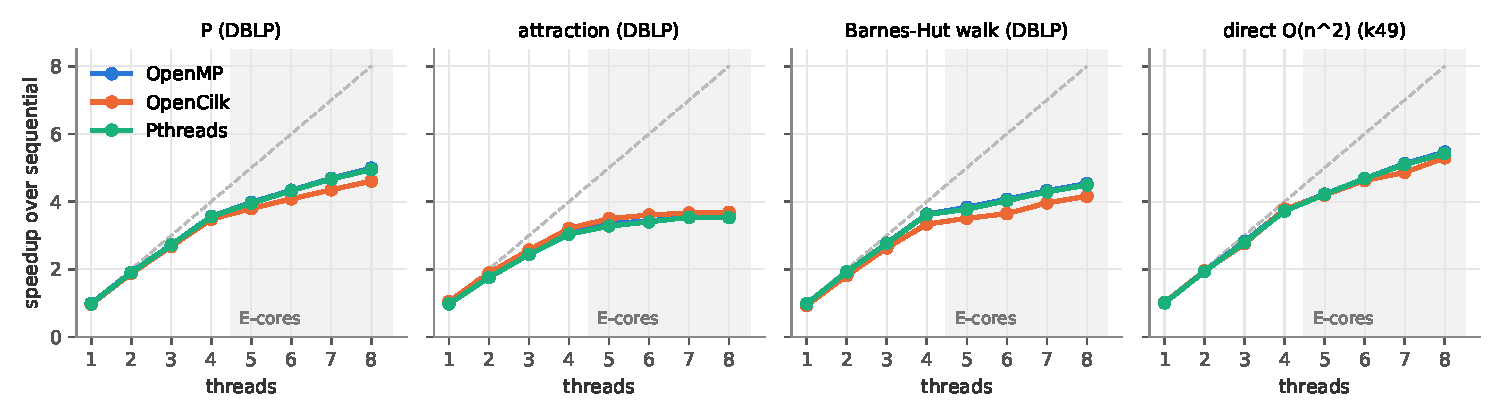
\includegraphics[width=\textwidth]{../figures/speedup.pdf}
\caption{\en{Speedup} σε σχέση με τον σειριακό κώδικα (\en{OpenMP} και \en{Pthreads} με
\en{dynamic,256}, \en{Cilk} με \en{work stealing}). Γκρι ζώνη: \en{threads} που τρέχουν σε
\en{efficiency} πυρήνες. Διακεκομμένη: ιδανικό.}
\label{fig:speedup}
\end{figure}

\textbf{Κλιμάκωση (Σχ.~\ref{fig:speedup}).} Μέχρι τα 4 \en{threads} οι καμπύλες είναι σχεδόν
γραμμικές: στο \en{DBLP} ο $P$ φτάνει $3.56\times$, το \en{walk} $3.63\times$, και ο άμεσος
υπολογισμός στο \texttt{k49} $3.76\times$. Μετά τα 4 η κλίση πέφτει, γιατί τα επιπλέον \en{threads}
πέφτουν σε \en{efficiency} πυρήνες. Από τον άμεσο υπολογισμό, που είναι καθαρά αριθμητικές πράξεις,
οι 4 \en{E-cores} προσθέτουν $5.46-3.76\approx1.7$ \en{P-cores}, άρα ένας \en{E-core} αξίζει περίπου
το 0.4 ενός \en{P-core}. Στα 8 \en{threads}: $P$ $4.99\times$, \en{walk} $4.53\times$, άμεσος
$5.46\times$. Η έλξη σταματά κοντά στο $3.5\times$: ανά ακμή κάνει λίγες πράξεις και μία τυχαία
ανάγνωση του $y_j$, οπότε την περιορίζει η μνήμη και όχι οι πυρήνες. Η κατασκευή του δέντρου
($<2\%$ του χρόνου) φτάνει το πολύ $2.3\times$ (\en{Amazon}) και δεν κερδίζει τίποτα στο
\texttt{k49} (1.2\,\en{ms}): ο χωρισμός της ρίζας και το περικλείον τετράγωνο είναι σειριακά και
περνούν από όλα τα $n$ σημεία, και κάτω από το όριο δεν δημιουργούνται \en{tasks} (\en{Amdahl}). Τα
τρία μοντέλα απέχουν λίγες μονάδες τοις εκατό μεταξύ τους. Το \en{Cilk} υστερεί λίγο στο
\en{walk} (και με 1 \en{worker}, άρα φταίει ο κώδικας του \en{clang} και όχι ο \en{scheduler}). Ένα
σαφές κόστος του δικού μου σχεδιασμού στα \en{Pthreads}: με \en{dynamic scheduling} η κλίση
(0.6\,\en{ms} στο \en{Amazon}) γίνεται 2.8\,\en{ms} στα 8 \en{threads}, ενώ με \en{static} μένει
0.57\,\en{ms}. Κάθε επανάληψη είναι μία αφαίρεση, οπότε με 2\,600 κομμάτια των 256 τα \en{threads}
κυρίως ανταγωνίζονται για τον κοινό \en{atomic} μετρητή. Ένα δυναμικό κομμάτι πρέπει να είναι
μεγάλο σε σχέση με τη δουλειά που μοιράζει.

\begin{figure}[t]
\centering
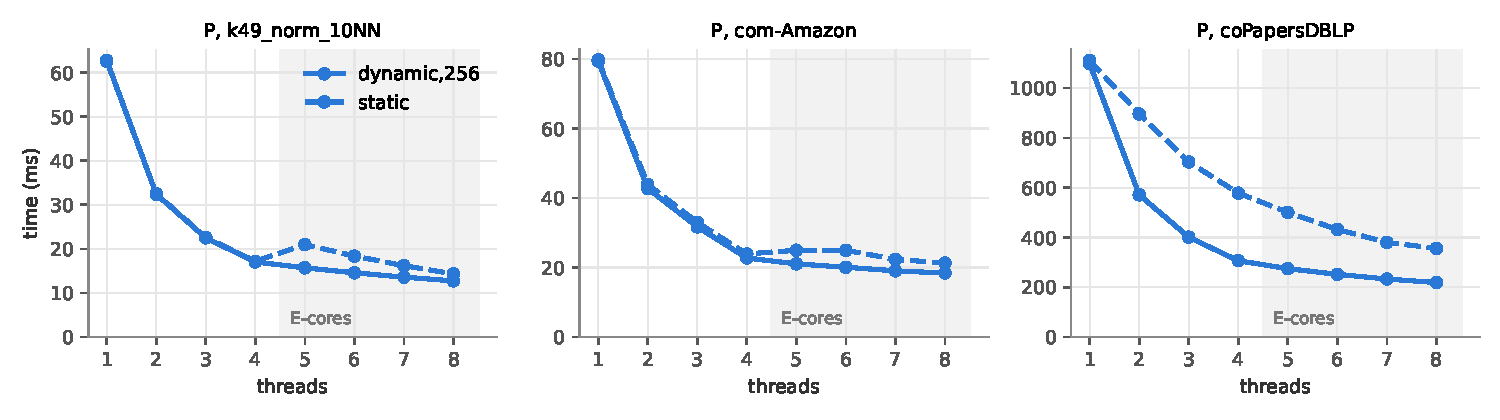
\includegraphics[width=\textwidth]{../figures/schedule.pdf}
\caption{Φάση $P$ με \en{OpenMP}, \en{static} έναντι \en{dynamic,256} \en{scheduling}.}
\label{fig:schedule}
\end{figure}

\textbf{\en{Static} έναντι \en{dynamic} (Σχ.~\ref{fig:schedule}).} Στα \texttt{k49} και \en{Amazon}
το \en{static} είναι εξίσου καλό με το \en{dynamic} μέχρι τα 4 \en{threads}, και χάνει μόνο όταν ένα
\en{block} πέφτει σε \en{E-core} (13--16\% στα 8 \en{threads}): όλοι περιμένουν τον αργό πυρήνα. Στο
\en{DBLP} το \en{static} είναι ήδη $1.57\times$ πιο αργό στα 2 \en{threads} και $1.89\times$ στα 4,
μόνο με \en{P-cores}. Το κόστος μιας γραμμής είναι ανάλογο του βαθμού της (από 1 έως 3\,299). Το
πιθανότερο είναι ότι οι βαθμοί δεν είναι ομοιόμορφα κατανεμημένοι στην αρίθμηση των κόμβων, άρα
ίσα \en{blocks} γραμμών δεν είναι ίση δουλειά, και τα δυναμικά κομμάτια των 256 γραμμών το
εξισορροπούν. Το \en{walk} δεν το δείχνει αυτό, αφού το κόστος του εξαρτάται από την πυκνότητα των
σημείων και όχι από τους βαθμούς. Στον άμεσο υπολογισμό (0.45\,\en{s}) το \en{static} και το
\en{dynamic} έδωσαν τον ίδιο χρόνο ακόμα και στα 5--8 \en{threads}. Η εξήγησή μου, που δεν την έχω
επαληθεύσει, είναι ότι σε μια τόσο μεγάλη φάση το \en{macOS} προλαβαίνει να μετακινεί τα \en{threads}
ανάμεσα στα είδη πυρήνων.

\textbf{\en{Barnes--Hut} έναντι άμεσου.} Στο \texttt{k49} το \en{Barnes--Hut}
(\en{build+centres+walk}) είναι $22\times$ ταχύτερο από τον άμεσο υπολογισμό σειριακά (86\,\en{ms}
έναντι 1.91\,\en{s}) και $19\times$ στα 8 \en{threads}. Με άμεσο $\approx a n^2$ και
\en{Barnes--Hut} $\approx b\,n\log_2 n$, και τα $a,b$ προσαρμοσμένα στο \texttt{k49}, οι δύο
συναντιούνται στο $n\approx1\,200$. Κάτω από αυτό ο άμεσος υπολογισμός είναι ταχύτερος.

\textbf{Ανάμεσα στους γράφους (Σχ.~\ref{fig:phases}).} Ο $P$ και το \en{walk} παίρνουν πάνω από το
95\% του χρόνου σε κάθε γράφο. Από το \en{Amazon} στο \en{DBLP} το $n$ μεγαλώνει $1.6\times$ και το
\en{nnz} $16.5\times$: οι φάσεις των ακμών ακολουθούν το \en{nnz} ($P$ $13.7\times$, έλξη
$12.4\times$), το \en{walk} ακολουθεί το $n$ ($1.45\times$), και η κατασκευή και τα κέντρα μάζας
μεγαλώνουν γρηγορότερα από το $n$ ($2.9\times$, $3.6\times$) εξαιτίας των αλυσίδων από ταυτισμένα
σημεία.

\begin{figure}[t]
\centering
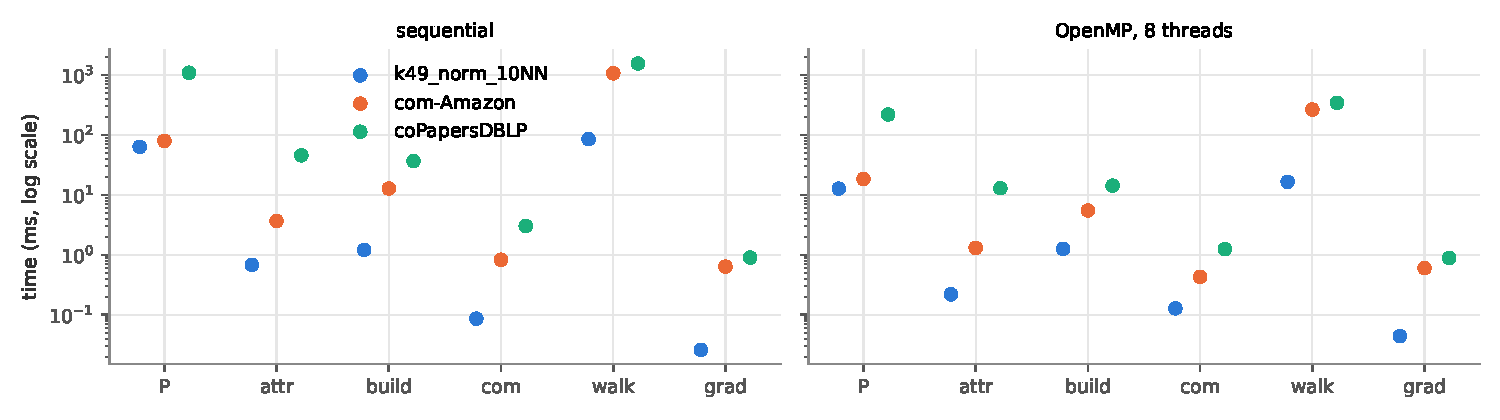
\includegraphics[width=\textwidth]{../figures/phases.pdf}
\caption{Χρόνος κάθε φάσης ανά γράφο, σειριακά και με \en{OpenMP} με 8 \en{threads}
(λογαριθμική κλίμακα).}
\label{fig:phases}
\end{figure}

\section{Πρόβλεψη για το \en{coPapersDBLP}}

Πριν τρέξω το \en{DBLP} στο \en{M1}, προέβλεψα κάθε φάση από τους χρόνους του \en{Amazon} στο ίδιο
μηχάνημα (η πρόβλεψη έγινε \en{commit} πριν από την εκτέλεση: \texttt{report/prediction-dblp.md}).
Μοντέλο: ο $P$ και η έλξη $\propto\mathrm{nnz}$ ($16.5\times$), η κατασκευή και το \en{walk}
$\propto n\log(n/m)$ ($1.69\times$), τα κέντρα μάζας και η κλίση $\propto n$. Οι παράλληλοι χρόνοι
είναι αυτοί διαιρεμένοι με το \en{speedup} του \en{Amazon}. (Το \en{DBLP} είχε τρέξει σειριακά στο
\en{Codespace} κατά την ανάπτυξη, αλλά δεν χρησιμοποίησα εκείνους τους χρόνους.)

\begin{table}[h]
\centering\small
\begin{tabular}{@{}lrrrrrr@{}}
\toprule
 & \multicolumn{2}{c}{σειριακά} & \multicolumn{2}{c}{4 \en{threads}} & \multicolumn{2}{c}{8 \en{threads}}\\
φάση & πρόβλεψη & μέτρηση & πρόβλεψη & μέτρηση & πρόβλεψη & μέτρηση \\
\midrule
$P$          & 1.31   & 1.093  & 0.37  & 0.307 & 0.30  & 0.219 \\
έλξη         & 0.061  & 0.046  & 0.022 & 0.015 & 0.022 & 0.013 \\
κατασκευή    & 0.022  & 0.037  & 0.010 & 0.016 & 0.009 & 0.014 \\
\en{walk}    & 1.81   & 1.553  & 0.55  & 0.428 & 0.45  & 0.343 \\
σύνολο (και οι έξι φάσεις) & 3.2 & 2.73 & 0.96 & 0.77 & 0.78 & 0.59 \\
\bottomrule
\end{tabular}
\caption{Δευτερόλεπτα, \en{OpenMP dynamic,256}. Το σύνολο προβλέφθηκε μεγαλύτερο κατά 17\% / 25\% /
32\%.}
\vspace{-4pt}
\end{table}

Για τον $P$, την έλξη και το \en{walk} η πρόβλεψη έδωσε περισσότερο χρόνο από τον πραγματικό: οι
γραμμές του \en{DBLP} είναι 10 φορές μεγαλύτερες (μέσος βαθμός 56 έναντι 5.5), οπότε υπάρχει
περισσότερη συνεχόμενη δουλειά ανά \en{cache miss} απ' ό,τι στο \en{Amazon}. Για τον ίδιο λόγο το
\en{DBLP} κλιμακώνεται καλύτερα ($P$: $4.99\times$ έναντι $4.32\times$ στα 8 \en{threads}), και γι'
αυτό το σφάλμα μεγαλώνει με το $p$. Για την κατασκευή και τα κέντρα μάζας η πρόβλεψη έδωσε
40--57\% λιγότερο χρόνο: τα ταυτισμένα σημεία του \en{DBLP} δίνουν 171\,223 κελιά, $2.7\times$ όσα
το \en{Amazon} αντί για $1.6\times$, με αλυσίδες κελιών με ένα παιδί μέχρι το βάθος 50.

\section{Ένα πραγματικό \en{bug}}

Οι πρώτες εκτελέσεις στο \en{M1} έδωσαν $5.6\times$ για τον $P$ και $6.2\times$ για το \en{walk}
με 4 \en{threads}, δηλαδή περισσότερο από τον αριθμό των \en{threads}, ενώ ο άμεσος υπολογισμός
έδωσε ακριβώς $4.0\times$. Δεν το πίστεψα. Τρέχοντας το σειριακό πρόγραμμα τρεις φορές στη σειρά
πήρα για τον $P$ 0.067, 0.066 και 0.064\,\en{s}, ενώ η πρώτη μέτρηση ήταν 0.096\,\en{s}, και η
\en{OpenMP} με 1 \en{thread} συμφωνούσε με τις «ζεστές» εκτελέσεις. Άρα το \en{bug} ήταν στη μέτρηση:
η σειριακή βάση έτρεξε πρώτη, με τον επεξεργαστή «κρύο», πριν ανέβει η συχνότητα. Ο άμεσος
υπολογισμός φαινόταν σωστός μόνο επειδή τρέχει τελευταίος μέσα στο πρόγραμμα. Η διόρθωση είναι η
εκτέλεση ζεστάματος που δεν καταγράφεται και οι σειριακές εκτελέσεις στην αρχή και στο τέλος στο
\texttt{scripts/measure.sh}. Τα διορθωμένα \en{speedup} είναι $3.8\times$ και $3.6\times$.

\section{Χρήση εργαλείων \en{AI}}

Χρησιμοποίησα το \en{Claude (Anthropic)} σε όλη την εργασία: για να μου εξηγήσει την εκφώνηση, για να
προτείνει τη δομή του κώδικα αρχείο προς αρχείο, για να γράψει τις πρώτες εκδόσεις των αρχείων
\en{C}, του \en{Makefile} και των \en{scripts} (\texttt{sweep\_m.sh}, \texttt{measure.sh},
\texttt{plots.py}), για να αναλύσει το \en{CSV} των χρόνων και την πρόβλεψη για το \en{DBLP}, και
για να γράψει ένα πρώτο κείμενο αυτής της αναφοράς. Έκανα \en{compile}, έτρεξα και έλεγξα κάθε βήμα
με τα αρχεία αναφοράς και ανάμεσα στις εκδόσεις. Λάθη του που χρειάστηκε να εντοπίσω ή που
διορθώθηκαν: έγραψε μια γραμμή για το \en{speedup} με τα \texttt{t0}/\texttt{t1} αφού είχαν
ξαναχρησιμοποιηθεί για άλλο χρονόμετρο, οπότε θα τύπωνε λάθος λόγο. Το πρώτο \en{script} μετρήσεων
τύπωνε τους χρόνους με 3 δεκαδικά, οπότε τα κέντρα μάζας και η κλίση έβγαιναν 0. Υπέθεσε ότι το
\en{Homebrew} εγκαθιστά τον \texttt{gcc-15}, ενώ ήταν ο \texttt{gcc-16}. Ένα \texttt{grep} που έδωσε
για τις σειριακές γραμμές του \en{CSV} δεν έβρισκε τίποτα. Το μοντέλο κόστους του για το \en{DBLP}
απείχε 17--37\% στις μεγάλες φάσεις και 40\% στην κατασκευή (ενότητα 6). Αρχικά εξήγησε το αργό
\en{gradient} των \en{Pthreads} με τη δημιουργία των \en{threads}, όμως οι εκτελέσεις με
\en{static}, που δημιουργούν τα ίδια \en{threads}, είναι γρήγορες, άρα η πραγματική αιτία είναι ο
ανταγωνισμός για τον μετρητή των κομματιών (ενότητα 5). Επίσης δεν προέβλεψε ούτε τα ταυτισμένα
σημεία ούτε την επίδραση του \en{static scheduling} στο \en{DBLP}. Και τα δύο βγήκαν από τις
μετρήσεις.

\end{document}
